\documentclass[a3paper,12pt]{extarticle} % Use extarticle for A3 paper size
\usepackage{graphicx} % Include this package for \includegraphics
\usepackage{amsmath}
\usepackage{amssymb} % Include this package for \mathbb
\usepackage[margin=1in]{geometry} % Adjust the margin as needed
\usepackage{float}
\usepackage{tikz} % Include this package for tikzpicture environment


\begin{document}

\author{kipngeno koech - bkoech}
\title{Homework 4 - Introduction to Probabilistic Graphical Models}   
\maketitle

\medskip

\maketitle

\section{Structure Learning}
\subsection{Tree-Selection and the Chow-Liu Algorithm}
Use the Chow-Liu Algorithm to learn the model (tree and parameters) that generated the following data.

\begin{figure}[H]
\centering
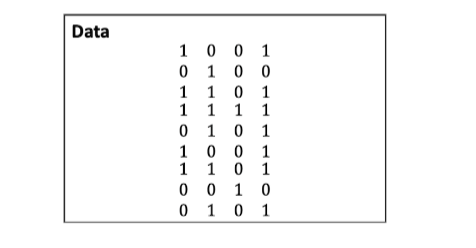
\includegraphics[width=0.8\textwidth]{q1.png}
\caption{The tree structure of the data.}
\label{fig:tree}
\end{figure}

The formula for calculating mutual information between the variables is:
\[
I(X;Y) = \sum_{x \in X} \sum_{y \in Y} p(x,y) \log\left(\frac{p(x,y)}{p(x)p(y)}\right)
\]
where \( p(x,y) \) is the joint probability of \( X \) and \( Y \), and \( p(x) \) and \( p(y) \) are the marginal probabilities of \( X \) and \( Y \), respectively.
The Chow-Liu algorithm is a method for constructing a maximum spanning tree (MST) from a set of variables based on their mutual information. The algorithm works as follows:
\begin{enumerate}
    \item Compute the mutual information \( I(X_i; X_j) \) for all pairs of variables \( (X_i, X_j) \).
    \item Create a weighted graph where each variable is a node and the edges are weighted by the mutual information values.
    \item Find the maximum spanning tree (MST) of the graph using Kruskal's or Prim's algorithm.
    \item The resulting tree structure represents the dependencies between the variables.
    \item Estimate the parameters of the tree structure using maximum likelihood estimation (MLE) or Bayesian methods.
    \item The resulting tree structure and parameters can be used for probabilistic inference and prediction.
\end{enumerate}
We need to compute the mutual information for all pairs of variables:
\begin{enumerate}
    \item \( I(X_1; X_2)\)
    \item \( I(X_1; X_3) \)
    \item \( I(X_2; X_3) \)
    \item \( I(X_1; X_4) \)
    \item \( I(X_2; X_4) \)
    \item \( I(X_3; X_4) \)
\end{enumerate}
\begin{enumerate}
    \item \( I(X_1; X_2) \)
let us start with the first one:
\begin{align*}
I(X_1; X_2) &= \sum_{x_1 \in X_1} \sum_{x_2 \in X_2} p(x_1,x_2) \log\left(\frac{p(x_1,x_2)}{p(x_1)p(x_2)}\right)\\
&= \sum_{x_1 \in X_1} \sum_{x_2 \in X_2} p(x_1,x_2) \log\left(\frac{p(x_1,x_2)}{p(x_1)p(x_2)}\right)\\
\end{align*}
so \(P(x_1, x_2)\) = (0,0), (0,1), (1,0), (1,1):
The mutual information is defined as:
\[
I(X_1; X_2) = \sum_{x_1 \in \{0,1\}} \sum_{x_2 \in \{0,1\}} P(x_1, x_2) \log_2 \left( \frac{P(x_1, x_2)}{P(x_1)P(x_2)} \right)
\]
Count the occurrences of each combination \((X_1 = x_1, X_2 = x_2)\):
\begin{itemize}
    \item \(X_1 = 0, X_2 = 0\): Occurs in 1 sample (row 8).
    \[
    P(X_1 = 0, X_2 = 0) = \frac{1}{9}
    \]
    \item \(X_1 = 0, X_2 = 1\): Occurs in 3 samples (rows 2, 5, 9).
    \[
    P(X_1 = 0, X_2 = 1) = \frac{3}{9} = \frac{1}{3}
    \]
    \item \(X_1 = 1, X_2 = 0\): Occurs in 2 samples (rows 1, 6).
    \[
    P(X_1 = 1, X_2 = 0) = \frac{2}{9}
    \]
    \item \(X_1 = 1, X_2 = 1\): Occurs in 3 samples (rows 3, 4, 7).
    \[
    P(X_1 = 1, X_2 = 1) = \frac{3}{9} = \frac{1}{3}
    \]
\end{itemize}
Verify: \(\frac{1}{9} + \frac{1}{3} + \frac{2}{9} + \frac{1}{3} = \frac{1 + 3 + 2 + 3}{9} = 1\).
Compute marginals:
\begin{itemize}
    \item For \(X_1\):
    \[
    P(X_1 = 0) = \frac{\text{4 samples (rows 2, 5, 8, 9)}}{9} = \frac{4}{9}, \quad P(X_1 = 1) = \frac{\text{5 samples (rows 1, 3, 4, 6, 7)}}{9} = \frac{5}{9}
    \]
    \item For \(X_2\):
    \[
    P(X_2 = 0) = \frac{\text{3 samples (rows 1, 6, 8)}}{9} = \frac{1}{3}, \quad P(X_2 = 1) = \frac{\text{6 samples (rows 2, 3, 4, 5, 7, 9)}}{9} = \frac{2}{3}
    \]
\end{itemize}

Computing the Mutual Information Terms\\
For each \((x_1, x_2)\), compute:
\[
P(x_1, x_2) \log_2 \left( \frac{P(x_1, x_2)}{P(x_1)P(x_2)} \right)
\]
\begin{itemize}
    \item \((x_1 = 0, x_2 = 0)\):
    \[
    P(X_1 = 0)P(X_2 = 0) = \frac{4}{9} \cdot \frac{1}{3} = \frac{4}{27}, \quad \frac{P(X_1 = 0, X_2 = 0)}{P(X_1 = 0)P(X_2 = 0)} = \frac{1/9}{4/27} = \frac{3}{4}
    \]
    \[
    \log_2 \left( \frac{3}{4} \right) \approx -0.415, \quad \text{Term} = \frac{1}{9} \cdot (-0.415) \approx -0.046
    \]
    \item \((x_1 = 0, x_2 = 1)\):
    \[
    P(X_1 = 0)P(X_2 = 1) = \frac{4}{9} \cdot \frac{2}{3} = \frac{8}{27}, \quad \frac{P(X_1 = 0, X_2 = 1)}{P(X_1 = 0)P(X_2 = 1)} = \frac{1/3}{8/27} = \frac{9}{8}
    \]
    \[
    \log_2 \left( \frac{9}{8} \right) \approx 0.170, \quad \text{Term} = \frac{1}{3} \cdot 0.170 \approx 0.057
    \]
    \item \((x_1 = 1, x_2 = 0)\):
    \[
    P(X_1 = 1)P(X_2 = 0) = \frac{5}{9} \cdot \frac{1}{3} = \frac{5}{27}, \quad \frac{P(X_1 = 1, X_2 = 0)}{P(X_1 = 1)P(X_2 = 0)} = \frac{2/9}{5/27} = \frac{6}{5}
    \]
    \[
    \log_2 \left( \frac{6}{5} \right) \approx 0.263, \quad \text{Term} = \frac{2}{9} \cdot 0.263 \approx 0.058
    \]
    \item \((x_1 = 1, x_2 = 1)\):
    \[
    P(X_1 = 1)P(X_2 = 1) = \frac{5}{9} \cdot \frac{2}{3} = \frac{10}{27}, \quad \frac{P(X_1 = 1, X_2 = 1)}{P(X_1 = 1)P(X_2 = 1)} = \frac{1/3}{10/27} = \frac{9}{10}
    \]
    \[
    \log_2 \left( \frac{9}{10} \right) \approx -0.152, \quad \text{Term} = \frac{1}{3} \cdot (-0.152) \approx -0.051
    \]
\end{itemize}

Sum the Terms:\\
Compute the mutual information:
\[
I(X_1; X_2) = (-0.046) + 0.057 + 0.058 - 0.051 \approx 0.018
\]

Thus, the mutual information is:
\[
I(X_1; X_2) \approx 0.018 \text{ bits}
\]

This value represents the weight of the edge between \(X_1\) and \(X_2\) in the Chow-Liu algorithm's graph.
\item \(X_1; X_3\):
\begin{align}
I(X_1; X_3) &= \sum_{x_1 \in X_1} \sum_{x_3 \in X_3} p(x_1,x_3) \log\left(\frac{p(x_1,x_3)}{p(x_1)p(x_3)}\right)\\
&= \sum_{x_1 \in X_1} \sum_{x_3 \in X_3} p(x_1,x_3) \log\left(\frac{p(x_1,x_3)}{p(x_1)p(x_3)}\right)\\
\end{align}
Given a dataset with 9 samples and 4 binary variables (\(X_1, X_2, X_3, X_4\)), we compute the mutual information \(I(X_1; X_3)\) for the Chow-Liu algorithm.

The mutual information is:
\[
I(X_1; X_3) = \sum_{x_1 \in \{0,1\}} \sum_{x_3 \in \{0,1\}} P(x_1, x_3) \log_2 \left( \frac{P(x_1, x_3)}{P(x_1)P(x_3)} \right)
\]

\textbf{Compute Joint Probabilities}: Count occurrences of \((X_1 = x_1, X_3 = x_3)\):
\begin{itemize}
    \item \(X_1 = 0, X_3 = 0\): 3 samples (rows 2, 5, 9).
    \[
    P(X_1 = 0, X_3 = 0) = \frac{3}{9} = \frac{1}{3}
    \]
    \item \(X_1 = 0, X_3 = 1\): 1 sample (row 8).
    \[
    P(X_1 = 0, X_3 = 1) = \frac{1}{9}
    \]
    \item \(X_1 = 1, X_3 = 0\): 4 samples (rows 1, 3, 6, 7).
    \[
    P(X_1 = 1, X_3 = 0) = \frac{4}{9}
    \]
    \item \(X_1 = 1, X_3 = 1\): 1 sample (row 4).
    \[
    P(X_1 = 1, X_3 = 1) = \frac{1}{9}
    \]
\end{itemize}
Verify: \(\frac{1}{3} + \frac{1}{9} + \frac{4}{9} + \frac{1}{9} = \frac{3 + 1 + 4 + 1}{9} = 1\).

\textbf{Compute Marginal Probabilities}:
\begin{itemize}
    \item \(X_1\):
    \[
    P(X_1 = 0) = \frac{\text{4 samples (rows 2, 5, 8, 9)}}{9} = \frac{4}{9}, \quad P(X_1 = 1) = \frac{\text{5 samples (rows 1, 3, 4, 6, 7)}}{9} = \frac{5}{9}
    \]
    \item \(X_3\):
    \[
    P(X_3 = 0) = \frac{\text{7 samples (rows 1, 2, 3, 5, 6, 7, 9)}}{9} = \frac{7}{9}, \quad P(X_3 = 1) = \frac{\text{2 samples (rows 4, 8)}}{9} = \frac{2}{9}
    \]
\end{itemize}

\textbf{Compute Mutual Information Terms}:
For each \((x_1, x_3)\), compute \(P(x_1, x_3) \log_2 \left( \frac{P(x_1, x_3)}{P(x_1)P(x_3)} \right)\):
\begin{itemize}
    \item \((x_1 = 0, x_3 = 0)\):
    \[
    P(X_1 = 0)P(X_3 = 0) = \frac{4}{9} \cdot \frac{7}{9} = \frac{28}{81}, \quad \frac{P(X_1 = 0, X_3 = 0)}{P(X_1 = 0)P(X_3 = 0)} = \frac{1/3}{28/81} = \frac{27}{28}
    \]
    \[
    \log_2 \left( \frac{27}{28} \right) \approx -0.053, \quad \text{Term} = \frac{1}{3} \cdot (-0.053) \approx -0.018
    \]
    \item \((x_1 = 0, x_3 = 1)\):
    \[
    P(X_1 = 0)P(X_3 = 1) = \frac{4}{9} \cdot \frac{2}{9} = \frac{8}{81}, \quad \frac{P(X_1 = 0, X_3 = 1)}{P(X_1 = 0)P(X_3 = 1)} = \frac{1/9}{8/81} = \frac{9}{8}
    \]
    \[
    \log_2 \left( \frac{9}{8} \right) \approx 0.170, \quad \text{Term} = \frac{1}{9} \cdot 0.170 \approx 0.019
    \]
    \item \((x_1 = 1, x_3 = 0)\):
    \[
    P(X_1 = 1)P(X_3 = 0) = \frac{5}{9} \cdot \frac{7}{9} = \frac{35}{81}, \quad \frac{P(X_1 = 1, X_3 = 0)}{P(X_1 = 1)P(X_3 = 0)} = \frac{4/9}{35/81} = \frac{36}{35}
    \]
    \[
    \log_2 \left( \frac{36}{35} \right) \approx 0.042, \quad \text{Term} = \frac{4}{9} \cdot 0.042 \approx 0.019
    \]
    \item \((x_1 = 1, x_3 = 1)\):
    \[
    P(X_1 = 1)P(X_3 = 1) = \frac{5}{9} \cdot \frac{2}{9} = \frac{10}{81}, \quad \frac{P(X_1 = 1, X_3 = 1)}{P(X_1 = 1)P(X_3 = 1)} = \frac{1/9}{10/81} = \frac{9}{10}
    \]
    \[
    \log_2 \left( \frac{9}{10} \right) \approx -0.152, \quad \text{Term} = \frac{1}{9} \cdot (-0.152) \approx -0.017
    \]
\end{itemize}

\textbf{Sum the Terms}:
\[
I(X_1; X_3) = (-0.018) + 0.019 + 0.019 - 0.017 \approx 0.003
\]
\[
I(X_1; X_3) \approx 0.003 \text{ bits}
\]

This is the weight of the edge between \(X_1\) and \(X_3\) in the Chow-Liu algorithm's graph.
\item \(X_2, X_3\):

We compute the mutual information \(I(X_2; X_3)\) for the Chow-Liu algorithm using a dataset with 9 samples.

The mutual information is:
\[
I(X_2; X_3) = \sum_{x_2 \in \{0,1\}} \sum_{x_3 \in \{0,1\}} P(x_2, x_3) \log_2 \left( \frac{P(x_2, x_3)}{P(x_2)P(x_3)} \right)
\]

\textbf{Compute Joint Probabilities}: Count occurrences of \((X_2 = x_2, X_3 = x_3)\):
\begin{itemize}
    \item \(X_2 = 0, X_3 = 0\): 2 samples (rows 1, 6).
    \[
    P(X_2 = 0, X_3 = 0) = \frac{2}{9}
    \]
    \item \(X_2 = 0, X_3 = 1\): 1 sample (row 8).
    \[
    P(X_2 = 0, X_3 = 1) = \frac{1}{9}
    \]
    \item \(X_2 = 1, X_3 = 0\): 5 samples (rows 2, 3, 5, 7, 9).
    \[
    P(X_2 = 1, X_3 = 0) = \frac{5}{9}
    \]
    \item \(X_2 = 1, X_3 = 1\): 1 sample (row 4).
    \[
    P(X_2 = 1, X_3 = 1) = \frac{1}{9}
    \]
\end{itemize}
Verify: \(\frac{2}{9} + \frac{1}{9} + \frac{5}{9} + \frac{1}{9} = \frac{2 + 1 + 5 + 1}{9} = 1\).

\textbf{Compute Marginal Probabilities}:
\begin{itemize}
    \item \(X_2\):
    \[
    P(X_2 = 0) = \frac{\text{3 samples (rows 1, 6, 8)}}{9} = \frac{1}{3}, \quad P(X_2 = 1) = \frac{\text{6 samples (rows 2, 3, 4, 5, 7, 9)}}{9} = \frac{2}{3}
    \]
    \item \(X_3\):
    \[
    P(X_3 = 0) = \frac{\text{7 samples (rows 1, 2, 3, 5, 6, 7, 9)}}{9} = \frac{7}{9}, \quad P(X_3 = 1) = \frac{\text{2 samples (rows 4, 8)}}{9} = \frac{2}{9}
    \]
\end{itemize}

\textbf{Compute Mutual Information Terms}:
For each \((x_2, x_3)\), compute \(P(x_2, x_3) \log_2 \left( \frac{P(x_2, x_3)}{P(x_2)P(x_3)} \right)\):
\begin{itemize}
    \item \((x_2 = 0, x_3 = 0)\):
    \[
    P(X_2 = 0)P(X_3 = 0) = \frac{1}{3} \cdot \frac{7}{9} = \frac{7}{27}, \quad \frac{P(X_2 = 0, X_3 = 0)}{P(X_2 = 0)P(X_3 = 0)} = \frac{2/9}{7/27} = \frac{6}{7}
    \]
    \[
    \log_2 \left( \frac{6}{7} \right) \approx -0.222, \quad \text{Term} = \frac{2}{9} \cdot (-0.222) \approx -0.049
    \]
    \item \((x_2 = 0, x_3 = 1)\):
    \[
    P(X_2 = 0)P(X_3 = 1) = \frac{1}{3} \cdot \frac{2}{9} = \frac{2}{27}, \quad \frac{P(X_2 = 0, X_3 = 1)}{P(X_2 = 0)P(X_3 = 1)} = \frac{1/9}{2/27} = \frac{3}{2}
    \]
    \[
    \log_2 \left( \frac{3}{2} \right) \approx 0.585, \quad \text{Term} = \frac{1}{9} \cdot 0.585 \approx 0.065
    \]
    \item \((x_2 = 1, x_3 = 0)\):
    \[
    P(X_2 = 1)P(X_3 = 0) = \frac{2}{3} \cdot \frac{7}{9} = \frac{14}{27}, \quad \frac{P(X_2 = 1, X_3 = 0)}{P(X_2 = 1)P(X_3 = 0)} = \frac{5/9}{14/27} = \frac{15}{14}
    \]
    \[
    \log_2 \left( \frac{15}{14} \right) \approx 0.100, \quad \text{Term} = \frac{5}{9} \cdot 0.100 \approx 0.056
    \]
    \item \((x_2 = 1, x_3 = 1)\):
    \[
    P(X_2 = 1)P(X_3 = 1) = \frac{2}{3} \cdot \frac{2}{9} = \frac{4}{27}, \quad \frac{P(X_2 = 1, X_3 = 1)}{P(X_2 = 1)P(X_3 = 1)} = \frac{1/9}{4/27} = \frac{3}{4}
    \]
    \[
    \log_2 \left( \frac{3}{4} \right) \approx -0.415, \quad \text{Term} = \frac{1}{9} \cdot (-0.415) \approx -0.046
    \]
\end{itemize}

\textbf{Sum the Terms}:
\[
I(X_2; X_3) = (-0.049) + 0.065 + 0.056 - 0.046 \approx 0.026
\]
\[
I(X_2; X_3) \approx 0.026 \text{ bits}
\]

This is the weight of the edge between \(X_2\) and \(X_3\) in the Chow-Liu algorithm's graph.
\item \(X_1, X_4\):

We compute the mutual information \(I(X_1; X_4)\) for the Chow-Liu algorithm using a dataset with 9 samples.

The mutual information is:
\[
I(X_1; X_4) = \sum_{x_1 \in \{0,1\}} \sum_{x_4 \in \{0,1\}} P(x_1, x_4) \log_2 \left( \frac{P(x_1, x_4)}{P(x_1)P(x_4)} \right)
\]

\textbf{Compute Joint Probabilities}: Count occurrences of \((X_1 = x_1, X_4 = x_4)\):
\begin{itemize}
    \item \(X_1 = 0, X_4 = 0\): 1 sample (row 2).
    \[
    P(X_1 = 0, X_4 = 0) = \frac{1}{9}
    \]
    \item \(X_1 = 0, X_4 = 1\): 3 samples (rows 5, 8, 9).
    \[
    P(X_1 = 0, X_4 = 1) = \frac{3}{9} = \frac{1}{3}
    \]
    \item \(X_1 = 1, X_4 = 0\): 0 samples.
    \[
    P(X_1 = 1, X_4 = 0) = \frac{0}{9} = 0
    \]
    \item \(X_1 = 1, X_4 = 1\): 5 samples (rows 1, 3, 4, 6, 7).
    \[
    P(X_1 = 1, X_4 = 1) = \frac{5}{9}
    \]
\end{itemize}
Verify: \(\frac{1}{9} + \frac{1}{3} + 0 + \frac{5}{9} = \frac{1 + 3 + 0 + 5}{9} = 1\).

\textbf{Compute Marginal Probabilities}:
\begin{itemize}
    \item \(X_1\):
    \[
    P(X_1 = 0) = \frac{\text{4 samples (rows 2, 5, 8, 9)}}{9} = \frac{4}{9}, \quad P(X_1 = 1) = \frac{\text{5 samples (rows 1, 3, 4, 6, 7)}}{9} = \frac{5}{9}
    \]
    \item \(X_4\):
    \[
    P(X_4 = 0) = \frac{\text{2 samples (rows 2, 8)}}{9} = \frac{2}{9}, \quad P(X_4 = 1) = \frac{\text{7 samples (rows 1, 3, 4, 5, 6, 7, 9)}}{9} = \frac{7}{9}
    \]
\end{itemize}

\textbf{Compute Mutual Information Terms}:
For each \((x_1, x_4)\), compute \(P(x_1, x_4) \log_2 \left( \frac{P(x_1, x_4)}{P(x_1)P(x_4)} \right)\):
\begin{itemize}
    \item \((x_1 = 0, x_4 = 0)\):
    \[
    P(X_1 = 0)P(X_4 = 0) = \frac{4}{9} \cdot \frac{2}{9} = \frac{8}{81}, \quad \frac{P(X_1 = 0, X_4 = 0)}{P(X_1 = 0)P(X_4 = 0)} = \frac{1/9}{8/81} = \frac{9}{8}
    \]
    \[
    \log_2 \left( \frac{9}{8} \right) \approx 0.170, \quad \text{Term} = \frac{1}{9} \cdot 0.170 \approx 0.019
    \]
    \item \((x_1 = 0, x_4 = 1)\):
    \[
    P(X_1 = 0)P(X_4 = 1) = \frac{4}{9} \cdot \frac{7}{9} = \frac{28}{81}, \quad \frac{P(X_1 = 0, X_4 = 1)}{P(X_1 = 0)P(X_4 = 1)} = \frac{1/3}{28/81} = \frac{27}{28}
    \]
    \[
    \log_2 \left( \frac{27}{28} \right) \approx -0.053, \quad \text{Term} = \frac{1}{3} \cdot (-0.053) \approx -0.018
    \]
    \item \((x_1 = 1, x_4 = 0)\):
    \[
    P(X_1 = 1, X_4 = 0) = 0, \quad \text{Term} = 0
    \]
    \item \((x_1 = 1, x_4 = 1)\):
    \[
    P(X_1 = 1)P(X_4 = 1) = \frac{5}{9} \cdot \frac{7}{9} = \frac{35}{81}, \quad \frac{P(X_1 = 1, X_4 = 1)}{P(X_1 = 1)P(X_4 = 1)} = \frac{5/9}{35/81} = \frac{81}{63} = \frac{9}{7}
    \]
    \[
    \log_2 \left( \frac{9}{7} \right) \approx 0.364, \quad \text{Term} = \frac{5}{9} \cdot 0.364 \approx 0.202
    \]
\end{itemize}

\textbf{Sum the Terms}:
\[
I(X_1; X_4) = 0.019 - 0.018 + 0 + 0.202 \approx 0.203
\]
\[
I(X_1; X_4) \approx 0.203 \text{ bits}
\]

This is the weight of the edge between \(X_1\) and \(X_4\) in the Chow-Liu algorithm's graph.
\item \(X_2, X_4\):

We compute the mutual information \(I(X_2; X_4)\) for the Chow-Liu algorithm using a dataset with 9 samples.

The mutual information is:
\[
I(X_2; X_4) = \sum_{x_2 \in \{0,1\}} \sum_{x_4 \in \{0,1\}} P(x_2, x_4) \log_2 \left( \frac{P(x_2, x_4)}{P(x_2)P(x_4)} \right)
\]

\textbf{Compute Joint Probabilities}: Count occurrences of \((X_2 = x_2, X_4 = x_4)\):
\begin{itemize}
    \item \(X_2 = 0, X_4 = 0\): 1 sample (row 8).
    \[
    P(X_2 = 0, X_4 = 0) = \frac{1}{9}
    \]
    \item \(X_2 = 0, X_4 = 1\): 2 samples (rows 1, 6).
    \[
    P(X_2 = 0, X_4 = 1) = \frac{2}{9}
    \]
    \item \(X_2 = 1, X_4 = 0\): 1 sample (row 2).
    \[
    P(X_2 = 1, X_4 = 0) = \frac{1}{9}
    \]
    \item \(X_2 = 1, X_4 = 1\): 5 samples (rows 3, 4, 5, 7, 9).
    \[
    P(X_2 = 1, X_4 = 1) = \frac{5}{9}
    \]
\end{itemize}
Verify: \(\frac{1}{9} + \frac{2}{9} + \frac{1}{9} + \frac{5}{9} = \frac{1 + 2 + 1 + 5}{9} = 1\).

\textbf{Compute Marginal Probabilities}:
\begin{itemize}
    \item \(X_2\):
    \[
    P(X_2 = 0) = \frac{\text{3 samples (rows 1, 6, 8)}}{9} = \frac{1}{3}, \quad P(X_2 = 1) = \frac{\text{6 samples (rows 2, 3, 4, 5, 7, 9)}}{9} = \frac{2}{3}
    \]
    \item \(X_4\):
    \[
    P(X_4 = 0) = \frac{\text{2 samples (rows 2, 8)}}{9} = \frac{2}{9}, \quad P(X_4 = 1) = \frac{\text{7 samples (rows 1, 3, 4, 5, 6, 7, 9)}}{9} = \frac{7}{9}
    \]
\end{itemize}

\textbf{Compute Mutual Information Terms}:
For each \((x_2, x_4)\), compute \(P(x_2, x_4) \log_2 \left( \frac{P(x_2, x_4)}{P(x_2)P(x_4)} \right)\):
\begin{itemize}
    \item \((x_2 = 0, x_4 = 0)\):
    \[
    P(X_2 = 0)P(X_4 = 0) = \frac{1}{3} \cdot \frac{2}{9} = \frac{2}{27}, \quad \frac{P(X_2 = 0, X_4 = 0)}{P(X_2 = 0)P(X_4 = 0)} = \frac{1/9}{2/27} = \frac{3}{2}
    \]
    \[
    \log_2 \left( \frac{3}{2} \right) \approx 0.585, \quad \text{Term} = \frac{1}{9} \cdot 0.585 \approx 0.065
    \]
    \item \((x_2 = 0, x_4 = 1)\):
    \[
    P(X_2 = 0)P(X_4 = 1) = \frac{1}{3} \cdot \frac{7}{9} = \frac{7}{27}, \quad \frac{P(X_2 = 0, X_4 = 1)}{P(X_2 = 0)P(X_4 = 1)} = \frac{2/9}{7/27} = \frac{6}{7}
    \]
    \[
    \log_2 \left( \frac{6}{7} \right) \approx -0.222, \quad \text{Term} = \frac{2}{9} \cdot (-0.222) \approx -0.049
    \]
    \item \((x_2 = 1, x_4 = 0)\):
    \[
    P(X_2 = 1)P(X_4 = 0) = \frac{2}{3} \cdot \frac{2}{9} = \frac{4}{27}, \quad \frac{P(X_2 = 1, X_4 = 0)}{P(X_2 = 1)P(X_4 = 0)} = \frac{1/9}{4/27} = \frac{3}{4}
    \]
    \[
    \log_2 \left( \frac{3}{4} \right) \approx -0.415, \quad \text{Term} = \frac{1}{9} \cdot (-0.415) \approx -0.046
    \]
    \item \((x_2 = 1, x_4 = 1)\):
    \[
    P(X_2 = 1)P(X_4 = 1) = \frac{2}{3} \cdot \frac{7}{9} = \frac{14}{27}, \quad \frac{P(X_2 = 1, X_4 = 1)}{P(X_2 = 1)P(X_4 = 1)} = \frac{5/9}{14/27} = \frac{15}{14}
    \]
    \[
    \log_2 \left( \frac{15}{14} \right) \approx 0.100, \quad \text{Term} = \frac{5}{9} \cdot 0.100 \approx 0.056
    \]
\end{itemize}

\textbf{Sum the Terms}:
\[
I(X_2; X_4) = 0.065 - 0.049 - 0.046 + 0.056 \approx 0.026
\]
\[
I(X_2; X_4) \approx 0.026 \text{ bits}
\]
\item \(X_3, X_4\):

We compute the mutual information \(I(X_3; X_4)\) for the Chow-Liu algorithm using a dataset with 9 samples.

The mutual information is:
\[
I(X_3; X_4) = \sum_{x_3 \in \{0,1\}} \sum_{x_4 \in \{0,1\}} P(x_3, x_4) \log_2 \left( \frac{P(x_3, x_4)}{P(x_3)P(x_4)} \right)
\]

\textbf{Compute Joint Probabilities}: Count occurrences of \((X_3 = x_3, X_4 = x_4)\):
\begin{itemize}
    \item \(X_3 = 0, X_4 = 0\): 1 sample (row 2).
    \[
    P(X_3 = 0, X_4 = 0) = \frac{1}{9}
    \]
    \item \(X_3 = 0, X_4 = 1\): 6 samples (rows 1, 3, 5, 6, 7, 9).
    \[
    P(X_3 = 0, X_4 = 1) = \frac{6}{9} = \frac{2}{3}
    \]
    \item \(X_3 = 1, X_4 = 0\): 1 sample (row 8).
    \[
    P(X_3 = 1, X_4 = 0) = \frac{1}{9}
    \]
    \item \(X_3 = 1, X_4 = 1\): 1 sample (row 4).
    \[
    P(X_3 = 1, X_4 = 1) = \frac{1}{9}
    \]
\end{itemize}
Verify: \(\frac{1}{9} + \frac{2}{3} + \frac{1}{9} + \frac{1}{9} = \frac{1 + 6 + 1 + 1}{9} = 1\).

\textbf{Compute Marginal Probabilities}:
\begin{itemize}
    \item \(X_3\):
    \[
    P(X_3 = 0) = \frac{\text{7 samples (rows 1, 2, 3, 5, 6, 7, 9)}}{9} = \frac{7}{9}, \quad P(X_3 = 1) = \frac{\text{2 samples (rows 4, 8)}}{9} = \frac{2}{9}
    \]
    \item \(X_4\):
    \[
    P(X_4 = 0) = \frac{\text{2 samples (rows 2, 8)}}{9} = \frac{2}{9}, \quad P(X_4 = 1) = \frac{\text{7 samples (rows 1, 3, 4, 5, 6, 7, 9)}}{9} = \frac{7}{9}
    \]
\end{itemize}

\textbf{Compute Mutual Information Terms}:
For each \((x_3, x_4)\), compute \(P(x_3, x_4) \log_2 \left( \frac{P(x_3, x_4)}{P(x_3)P(x_4)} \right)\):
\begin{itemize}
    \item \((x_3 = 0, x_4 = 0)\):
    \[
    P(X_3 = 0)P(X_4 = 0) = \frac{7}{9} \cdot \frac{2}{9} = \frac{14}{81}, \quad \frac{P(X_3 = 0, X_4 = 0)}{P(X_3 = 0)P(X_4 = 0)} = \frac{1/9}{14/81} = \frac{81}{126} = \frac{9}{14}
    \]
    \[
    \log_2 \left( \frac{9}{14} \right) \approx -0.637, \quad \text{Term} = \frac{1}{9} \cdot (-0.637) \approx -0.071
    \]
    \item \((x_3 = 0, x_4 = 1)\):
    \[
    P(X_3 = 0)P(X_4 = 1) = \frac{7}{9} \cdot \frac{7}{9} = \frac{49}{81}, \quad \frac{P(X_3 = 0, X_4 = 1)}{P(X_3 = 0)P(X_4 = 1)} = \frac{2/3}{49/81} = \frac{54}{49} = \frac{54}{49}
    \]
    \[
    \log_2 \left( \frac{54}{49} \right) \approx 0.139, \quad \text{Term} = \frac{2}{3} \cdot 0.139 \approx 0.093
    \]
    \item \((x_3 = 1, x_4 = 0)\):
    \[
    P(X_3 = 1)P(X_4 = 0) = \frac{2}{9} \cdot \frac{2}{9} = \frac{4}{81}, \quad \frac{P(X_3 = 1, X_4 = 0)}{P(X_3 = 1)P(X_4 = 0)} = \frac{1/9}{4/81} = \frac{81}{36} = \frac{9}{4}
    \]
    \[
    \log_2 \left( \frac{9}{4} \right) \approx 1.170, \quad \text{Term} = \frac{1}{9} \cdot 1.170 \approx 0.130
    \]
    \item \((x_3 = 1, x_4 = 1)\):
    \[
    P(X_3 = 1)P(X_4 = 1) = \frac{2}{9} \cdot \frac{7}{9} = \frac{14}{81}, \quad \frac{P(X_3 = 1, X_4 = 1)}{P(X_3 = 1)P(X_4 = 1)} = \frac{1/9}{14/81} = \frac{81}{126} = \frac{9}{14}
    \]
    \[
    \log_2 \left( \frac{9}{14} \right) \approx -0.637, \quad \text{Term} = \frac{1}{9} \cdot (-0.637) \approx -0.071
    \]
\end{itemize}

\textbf{Sum the Terms}:
\[
I(X_3; X_4) = (-0.071) + 0.093 + 0.130 - 0.071 \approx 0.081
\]
\[
I(X_3; X_4) \approx 0.081 \text{ bits}
\]
\item \textbf{Step 2: Constructing a Weighted Graph}

We construct a complete undirected graph with nodes \(X_1, X_2, X_3, X_4\), where each edge \((X_i, X_j)\) is weighted by the mutual information \(I(X_i; X_j)\).

\textbf{Graph Representation}:
\[
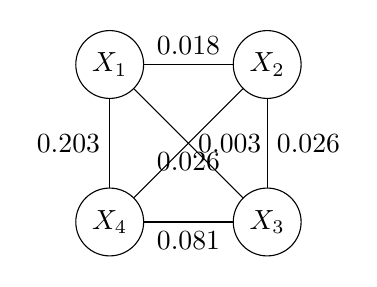
\begin{tikzpicture}
    % Nodes
    \node[circle, draw] (X1) at (0,2) {$X_1$};
    \node[circle, draw] (X2) at (2,2) {$X_2$};
    \node[circle, draw] (X3) at (2,0) {$X_3$};
    \node[circle, draw] (X4) at (0,0) {$X_4$};
    % Edges with weights
    \draw (X1) -- (X2) node[midway, above] {0.018};
    \draw (X1) -- (X3) node[midway, right] {0.003};
    \draw (X1) -- (X4) node[midway, left] {0.203};
    \draw (X2) -- (X3) node[midway, right] {0.026};
    \draw (X2) -- (X4) node[midway, below] {0.026};
    \draw (X3) -- (X4) node[midway, below] {0.081};
\end{tikzpicture}
\]

\item \textbf{Step 3: Finding the Maximum Spanning Tree}

We use Kruskal's algorithm to find the maximum spanning tree (MST) from the weighted graph, selecting edges that maximize the sum of mutual information while ensuring no cycles.

\textbf{Kruskal's Algorithm}:
\begin{enumerate}
    \item Sort edges by mutual information (descending order):
    \begin{itemize}
        \item \(X_1 - X_4\): 0.203
        \item \(X_3 - X_4\): 0.081
        \item \(X_2 - X_3\): 0.026
        \item \(X_2 - X_4\): 0.026
        \item \(X_1 - X_2\): 0.018
        \item \(X_1 - X_3\): 0.003
    \end{itemize}
    \item Initialize an empty tree.
    \item Add edges, skipping those that create cycles:
    \begin{itemize}
        \item Add \(X_1 - X_4\) (0.203): Connects \(X_1, X_4\), no cycle.
        \item Add \(X_3 - X_4\) (0.081): Connects \(X_3\) to \(X_4\), no cycle (\(X_1 - X_4 - X_3\)).
        \item Add \(X_2 - X_3\) (0.026): Connects \(X_2\) to \(X_3\), no cycle (\(X_1 - X_4 - X_3 - X_2\)).
        \item Skip \(X_2 - X_4\) (0.026): Creates cycle (\(X_2 - X_3 - X_4 - X_2\)).
        \item Skip \(X_1 - X_2\) (0.018): Creates cycle (\(X_1 - X_4 - X_3 - X_2 - X_1\)).
        \item Skip \(X_1 - X_3\) (0.003): Creates cycle (\(X_1 - X_4 - X_3 - X_1\)).
    \end{itemize}
    \item The tree has 3 edges, connecting all 4 nodes.
\end{enumerate}

\textbf{Maximum Spanning Tree}:
The MST includes edges:
\begin{itemize}
    \item \(X_1 - X_4\) (weight 0.203)
    \item \(X_3 - X_4\) (weight 0.081)
    \item \(X_2 - X_3\) (weight 0.026)
\end{itemize}
Total weight: \(0.203 + 0.081 + 0.026 \approx 0.310\).

\textbf{Visualization of the MST}:
\[
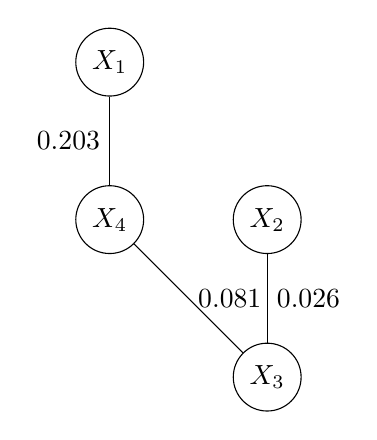
\begin{tikzpicture}
    % Nodes
    \node[circle, draw] (X1) at (0,2) {$X_1$};
    \node[circle, draw] (X2) at (2,0) {$X_2$};
    \node[circle, draw] (X3) at (2,-2) {$X_3$};
    \node[circle, draw] (X4) at (0,0) {$X_4$};
    % Edges with weights
    \draw (X1) -- (X4) node[midway, left] {0.203};
    \draw (X3) -- (X4) node[midway, right] {0.081};
    \draw (X2) -- (X3) node[midway, right] {0.026};
\end{tikzpicture}
\]
\item \textbf{Step 4: Direct the Edges}

We direct the edges of the maximum spanning tree to form a Bayesian network by choosing a root node and orienting edges away from it. We select \(X_4\) as the root.

The MST edges \(X_1 - X_4\), \(X_3 - X_4\), \(X_2 - X_3\) are directed as:
\begin{itemize}
    \item \(X_4 \to X_1\)
    \item \(X_4 \to X_3\)
    \item \(X_3 \to X_2\)
\end{itemize}

\textbf{Directed Tree Visualization}:
\[
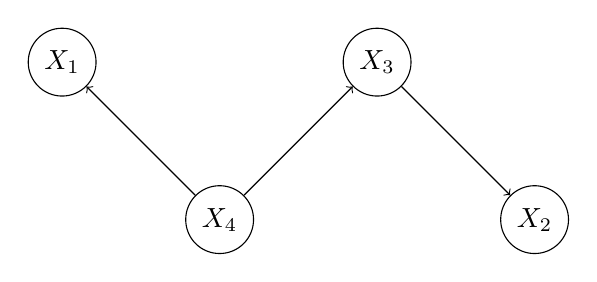
\begin{tikzpicture}
    % Nodes
    \node[circle, draw] (X4) at (0,0) {$X_4$};
    \node[circle, draw] (X1) at (-2,2) {$X_1$};
    \node[circle, draw] (X3) at (2,2) {$X_3$};
    \node[circle, draw] (X2) at (4,0) {$X_2$};
    % Directed edges
    \draw[->] (X4) -- (X1);
    \draw[->] (X4) -- (X3);
    \draw[->] (X3) -- (X2);
\end{tikzpicture}
\]

The joint distribution is:
\[
P(X_1, X_2, X_3, X_4) = P(X_4) P(X_1 | X_4) P(X_3 | X_4) P(X_2 | X_3)
\]

\item \textbf{Step 5: Parameter Estimation}

We estimate the conditional probabilities from the data (9 samples) by counting occurrences.

\textbf{1. \(P(X_4)\)} (root, no parent):
\begin{itemize}
    \item \(X_4 = 0\): 2 samples (rows 2, 8).
    \[
    P(X_4 = 0) = \frac{2}{9}
    \]
    \item \(X_4 = 1\): 7 samples (rows 1, 3, 4, 5, 6, 7, 9).
    \[
    P(X_4 = 1) = \frac{7}{9}
    \]
\end{itemize}

\textbf{2. \(P(X_1 | X_4)\)} (parent: \(X_4\)):
\begin{itemize}
    \item For \(X_4 = 0\) (2 samples: rows 2, 8):
    \[
    P(X_1 = 0 | X_4 = 0) = \frac{\text{2 samples (rows 2, 8)}}{2} = 1, \quad P(X_1 = 1 | X_4 = 0) = \frac{0}{2} = 0
    \]
    \item For \(X_4 = 1\) (7 samples: rows 1, 3, 4, 5, 6, 7, 9):
    \[
    P(X_1 = 0 | X_4 = 1) = \frac{\text{2 samples (rows 5, 9)}}{7} = \frac{2}{7}, \quad P(X_1 = 1 | X_4 = 1) = \frac{\text{5 samples (rows 1, 3, 4, 6, 7)}}{7} = \frac{5}{7}
    \]
\end{itemize}

\textbf{3. \(P(X_3 | X_4)\)} (parent: \(X_4\)):
\begin{itemize}
    \item For \(X_4 = 0\) (2 samples: rows 2, 8):
    \[
    P(X_3 = 0 | X_4 = 0) = \frac{\text{1 sample (row 2)}}{2} = \frac{1}{2}, \quad P(X_3 = 1 | X_4 = 0) = \frac{\text{1 sample (row 8)}}{2} = \frac{1}{2}
    \]
    \item For \(X_4 = 1\) (7 samples: rows 1, 3, 4, 5, 6, 7, 9):
    \[
    P(X_3 = 0 | X_4 = 1) = \frac{\text{6 samples (rows 1, 3, 5, 6, 7, 9)}}{7} = \frac{6}{7}, \quad P(X_3 = 1 | X_4 = 1) = \frac{\text{1 sample (row 4)}}{7} = \frac{1}{7}
    \]
\end{itemize}

\textbf{4. \(P(X_2 | X_3)\)} (parent: \(X_3\)):
\begin{itemize}
    \item For \(X_3 = 0\) (7 samples: rows 1, 2, 3, 5, 6, 7, 9):
    \[
    P(X_2 = 0 | X_3 = 0) = \frac{\text{2 samples (rows 1, 6)}}{7} = \frac{2}{7}, \quad P(X_2 = 1 | X_3 = 0) = \frac{\text{5 samples (rows 2, 3, 5, 7, 9)}}{7} = \frac{5}{7}
    \]
    \item For \(X_3 = 1\) (2 samples: rows 4, 8):
    \[
    P(X_2 = 0 | X_3 = 1) = \frac{\text{1 sample (row 8)}}{2} = \frac{1}{2}, \quad P(X_2 = 1 | X_3 = 1) = \frac{\text{1 sample (row 4)}}{2} = \frac{1}{2}
    \]
\end{itemize}

\textbf{Model Parameters}:
The Bayesian network is defined by:
\begin{itemize}
    \item \(P(X_4 = 0) = \frac{2}{9}\), \(P(X_4 = 1) = \frac{7}{9}\)
    \item \(P(X_1 = 0 | X_4 = 0) = 1\), \(P(X_1 = 1 | X_4 = 0) = 0\)
    \item \(P(X_1 = 0 | X_4 = 1) = \frac{2}{7}\), \(P(X_1 = 1 | X_4 = 1) = \frac{5}{7}\)
    \item \(P(X_3 = 0 | X_4 = 0) = \frac{1}{2}\), \(P(X_3 = 1 | X_4 = 0) = \frac{1}{2}\)
    \item \(P(X_3 = 0 | X_4 = 1) = \frac{6}{7}\), \(P(X_3 = 1 | X_4 = 1) = \frac{1}{7}\)
    \item \(P(X_2 = 0 | X_3 = 0) = \frac{2}{7}\), \(P(X_2 = 1 | X_3 = 0) = \frac{5}{7}\)
    \item \(P(X_2 = 0 | X_3 = 1) = \frac{1}{2}\), \(P(X_2 = 1 | X_3 = 1) = \frac{1}{2}\)
\end{itemize}


\end{enumerate}

\subsection{Scoring Function}
Using the BIC scoring metrics below, compute the model (graph and potentials) that generated the data below. 

\textbf{BIC:}
\[
S(G, \theta; D) = LL(\theta; D) - \phi(|D|)\|G\| \quad \text{where} \quad \phi(t) = \frac{\log(t)}{2}
\]

\textbf{Maximizing the score:}
\[
S_{\text{max}}(G, D) = \max_{\theta} \big(S(G, \theta; D)\big)
\]

\begin{figure}[H]
\centering
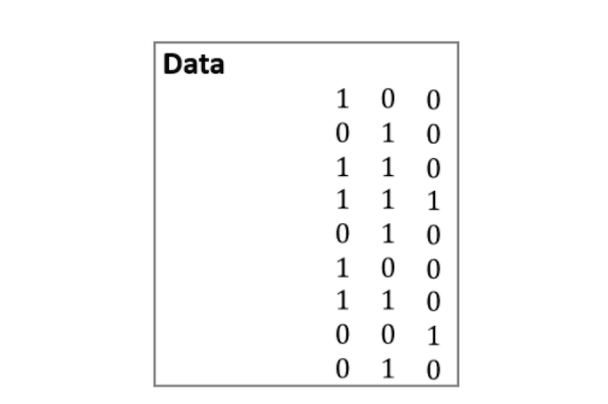
\includegraphics[width=0.8\textwidth]{q2.png}
\caption{The data used to compute the BIC score.}
\label{fig:data}
\end{figure}


We compute the Bayesian network (graph and parameters) that maximizes the BIC score for the given dataset with 9 samples and 3 binary variables (\(X_1, X_2, X_3\)). The BIC score is:

\[
S(G, \theta; D) = LL(\theta; D) - \frac{\log(9)}{2} \cdot \|G\|
\]

where \(LL(\theta; D)\) is the log-likelihood, \(\|G\|\) is the number of independent parameters, and \(\log(9) \approx 2.197\), so \(\frac{\log(9)}{2} \approx 1.099\). We evaluate five representative directed acyclic graphs (DAGs), compute their parameters, log-likelihood, and BIC scores, and select the graph with the highest score.

\textbf{Graphs Considered}:
\begin{itemize}
    \item \(G_1\): No edges (\(X_1, X_2, X_3\)).
    \item \(G_2\): \(X_1 \to X_2\).
    \item \(G_3\): \(X_1 \to X_2 \to X_3\).
    \item \(G_4\): \(X_1 \to X_2, X_1 \to X_3\).
    \item \(G_5\): \(X_1 \to X_2, X_1 \to X_3, X_2 \to X_3\).
\end{itemize}

\textbf{Graph \(G_1\): No Edges}

Joint distribution: \(P(X_1, X_2, X_3) = P(X_1)P(X_2)P(X_3)\).

Parameters:
\begin{itemize}
    \item \(X_1 = 0\): 4 samples (rows 2, 5, 8, 9).
    \[
    P(X_1 = 0) = \frac{4}{9}, \quad P(X_1 = 1) = \frac{5}{9}
    \]
    \item \(X_2 = 0\): 3 samples (rows 1, 6, 8).
    \[
    P(X_2 = 0) = \frac{1}{3}, \quad P(X_2 = 1) = \frac{2}{3}
    \]
    \item \(X_3 = 0\): 7 samples (rows 1, 2, 3, 5, 6, 7, 9).
    \[
    P(X_3 = 0) = \frac{7}{9}, \quad P(X_3 = 1) = \frac{2}{9}
    \]
\end{itemize}

Log-likelihood: \(LL(\theta; D) = \sum_{i=1}^9 \log P(x_i)\), where \(P(x_i) = P(X_1 = x_{i,1}) P(X_2 = x_{i,2}) P(X_3 = x_{i,3})\).

For each sample:
\begin{itemize}
    \item Row 1: \((1,0,0)\): \(P = \frac{5}{9} \cdot \frac{1}{3} \cdot \frac{7}{9} = \frac{35}{243}\), \(\log \frac{35}{243} \approx -1.936\)
    \item Row 2: \((0,1,0)\): \(P = \frac{4}{9} \cdot \frac{2}{3} \cdot \frac{7}{9} = \frac{56}{243}\), \(\log \frac{56}{243} \approx -1.467\)
    \item Row 3: \((1,1,0)\): \(P = \frac{5}{9} \cdot \frac{2}{3} \cdot \frac{7}{9} = \frac{70}{243}\), \(\log \frac{70}{243} \approx -1.246\)
    \item Row 4: \((1,1,1)\): \(P = \frac{5}{9} \cdot \frac{2}{3} \cdot \frac{2}{9} = \frac{20}{243}\), \(\log \frac{20}{243} \approx -2.497\)
    \item Row 5: \((0,1,0)\): Same as Row 2, \(\log \frac{56}{243} \approx -1.467\)
    \item Row 6: \((1,0,0)\): Same as Row 1, \(\log \frac{35}{243} \approx -1.936\)
    \item Row 7: \((1,1,0)\): Same as Row 3, \(\log \frac{70}{243} \approx -1.246\)
    \item Row 8: \((0,0,1)\): \(P = \frac{4}{9} \cdot \frac{1}{3} \cdot \frac{2}{9} = \frac{8}{243}\), \(\log \frac{8}{243} \approx -3.406\)
    \item Row 9: \((0,1,0)\): Same as Row 2, \(\log \frac{56}{243} \approx -1.467\)
\end{itemize}
Sum: \(LL(\theta; D) \approx -1.936 + (-1.467) + (-1.246) + (-2.497) + (-1.467) + (-1.936) + (-1.246) + (-3.406) + (-1.467) \approx -16.668\).

Parameters: \(\|G_1\| = 1 + 1 + 1 = 3\).

BIC Score:
\[
S(G_1, \theta; D) \approx -16.668 - 1.099 \cdot 3 \approx -16.668 - 3.297 \approx -19.965
\]

\textbf{Graph \(G_2\): \(X_1 \to X_2\)}

Joint distribution: \(P(X_1, X_2, X_3) = P(X_1)P(X_2 | X_1)P(X_3)\).

Parameters:
\begin{itemize}
    \item \(P(X_1)\): Same as \(G_1\), \(P(X_1 = 0) = \frac{4}{9}\), \(P(X_1 = 1) = \frac{5}{9}\).
    \item \(X_1 = 0\) (4 samples: rows 2, 5, 8, 9): \(X_2 = 0\): 1 (row 8), \(X_2 = 1\): 3 (rows 2, 5, 9).
    \[
    P(X_2 = 0 | X_1 = 0) = \frac{1}{4}, \quad P(X_2 = 1 | X_1 = 0) = \frac{3}{4}
    \]
    \item \(X_1 = 1\) (5 samples: rows 1, 3, 4, 6, 7): \(X_2 = 0\): 2 (rows 1, 6), \(X_2 = 1\): 3 (rows 3, 4, 7).
    \[
    P(X_2 = 0 | X_1 = 1) = \frac{2}{5}, \quad P(X_2 = 1 | X_1 = 1) = \frac{3}{5}
    \]
    \item \(P(X_3)\): Same as \(G_1\), \(P(X_3 = 0) = \frac{7}{9}\), \(P(X_3 = 1) = \frac{2}{9}\).
\end{itemize}

Log-likelihood: \(P(x_i) = P(X_1 = x_{i,1}) P(X_2 = x_{i,2} | X_1 = x_{i,1}) P(X_3 = x_{i,3})\).
\begin{itemize}
    \item Row 1: \((1,0,0)\): \(P = \frac{5}{9} \cdot \frac{2}{5} \cdot \frac{7}{9} = \frac{70}{405}\), \(\log \frac{70}{405} \approx -1.753\)
    \item Row 2: \((0,1,0)\): \(P = \frac{4}{9} \cdot \frac{3}{4} \cdot \frac{7}{9} = \frac{84}{324}\), \(\log \frac{84}{324} \approx -1.350\)
    \item Row 3: \((1,1,0)\): \(P = \frac{5}{9} \cdot \frac{3}{5} \cdot \frac{7}{9} = \frac{105}{405}\), \(\log \frac{105}{405} \approx -1.350\)
    \item Row 4: \((1,1,1)\): \(P = \frac{5}{9} \cdot \frac{3}{5} \cdot \frac{2}{9} = \frac{30}{405}\), \(\log \frac{30}{405} \approx -2.601\)
    \item Row 5: \((0,1,0)\): Same as Row 2, \(\log \frac{84}{324} \approx -1.350\)
    \item Row 6: \((1,0,0)\): Same as Row 1, \(\log \frac{70}{405} \approx -1.753\)
    \item Row 7: \((1,1,0)\): Same as Row 3, \(\log \frac{105}{405} \approx -1.350\)
    \item Row 8: \((0,0,1)\): \(P = \frac{4}{9} \cdot \frac{1}{4} \cdot \frac{2}{9} = \frac{8}{324}\), \(\log \frac{8}{324} \approx -3.689\)
    \item Row 9: \((0,1,0)\): Same as Row 2, \(\log \frac{84}{324} \approx -1.350\)
\end{itemize}
Sum: \(LL(\theta; D) \approx -1.753 + (-1.350) + (-1.350) + (-2.601) + (-1.350) + (-1.753) + (-1.350) + (-3.689) + (-1.350) \approx -16.546\).

Parameters: \(\|G_2\| = 1 + 2 + 1 = 4\).

BIC Score:
\[
S(G_2, \theta; D) \approx -16.546 - 1.099 \cdot 4 \approx -16.546 - 4.396 \approx -20.942
\]

\textbf{Graph \(G_3\): \(X_1 \to X_2 \to X_3\)}

Joint distribution: \(P(X_1, X_2, X_3) = P(X_1)P(X_2 | X_1)P(X_3 | X_2)\).

Parameters:
\begin{itemize}
    \item \(P(X_1)\): Same as \(G_1\).
    \item \(P(X_2 | X_1)\): Same as \(G_2\).
    \item \(X_2 = 0\) (3 samples: rows 1, 6, 8): \(X_3 = 0\): 2 (rows 1, 6), \(X_3 = 1\): 1 (row 8).
    \[
    P(X_3 = 0 | X_2 = 0) = \frac{2}{3}, \quad P(X_3 = 1 | X_2 = 0) = \frac{1}{3}
    \]
    \item \(X_2 = 1\) (6 samples: rows 2, 3, 4, 5, 7, 9): \(X_3 = 0\): 5 (rows 2, 3, 5, 7, 9), \(X_3 = 1\): 1 (row 4).
    \[
    P(X_3 = 0 | X_2 = 1) = \frac{5}{6}, \quad P(X_3 = 1 | X_2 = 1) = \frac{1}{6}
    \]
\end{itemize}

Log-likelihood: \(P(x_i) = P(X_1 = x_{i,1}) P(X_2 = x_{i,2} | X_1 = x_{i,1}) P(X_3 = x_{i,3} | X_2 = x_{i,2})\).
\begin{itemize}
    \item Row 1: \((1,0,0)\): \(P = \frac{5}{9} \cdot \frac{2}{5} \cdot \frac{2}{3} = \frac{20}{135}\), \(\log \frac{20}{135} \approx -1.911\)
    \item Row 2: \((0,1,0)\): \(P = \frac{4}{9} \cdot \frac{3}{4} \cdot \frac{5}{6} = \frac{60}{216}\), \(\log \frac{60}{216} \approx -1.279\)
    \item Row 3: \((1,1,0)\): \(P = \frac{5}{9} \cdot \frac{3}{5} \cdot \frac{5}{6} = \frac{75}{270}\), \(\log \frac{75}{270} \approx -1.279\)
    \item Row 4: \((1,1,1)\): \(P = \frac{5}{9} \cdot \frac{3}{5} \cdot \frac{1}{6} = \frac{15}{270}\), \(\log \frac{15}{270} \approx -2.890\)
    \item Row 5: \((0,1,0)\): Same as Row 2, \(\log \frac{60}{216} \approx -1.279\)
    \item Row 6: \((1,0,0)\): Same as Row 1, \(\log \frac{20}{135} \approx -1.911\)
    \item Row 7: \((1,1,0)\): Same as Row 3, \(\log \frac{75}{270} \approx -1.279\)
    \item Row 8: \((0,0,1)\): \(P = \frac{4}{9} \cdot \frac{1}{4} \cdot \frac{1}{3} = \frac{4}{108}\), \(\log \frac{4}{108} \approx -3.300\)
    \item Row 9: \((0,1,0)\): Same as Row 2, \(\log \frac{60}{216} \approx -1.279\)
\end{itemize}
Sum: \(LL(\theta; D) \approx -1.911 + (-1.279) + (-1.279) + (-2.890) + (-1.279) + (-1.911) + (-1.279) + (-3.300) + (-1.279) \approx -16.407\).

Parameters: \(\|G_3\| = 1 + 2 + 2 = 5\).

BIC Score:
\[
S(G_3, \theta; D) \approx -16.407 - 1.099 \cdot 5 \approx -16.407 - 5.495 \approx -21.902
\]

\textbf{Graph \(G_4\): \(X_1 \to X_2, X_1 \to X_3\)}

Joint distribution: \(P(X_1, X_2, X_3) = P(X_1)P(X_2 | X_1)P(X_3 | X_1)\).

Parameters:
\begin{itemize}
    \item \(P(X_1)\), \(P(X_2 | X_1)\): Same as \(G_2\).
    \item \(X_1 = 0\) (4 samples): \(X_3 = 0\): 3 (rows 2, 5, 9), \(X_3 = 1\): 1 (row 8).
    \[
    P(X_3 = 0 | X_1 = 0) = \frac{3}{4}, \quad P(X_3 = 1 | X_1 = 0) = \frac{1}{4}
    \]
    \item \(X_1 = 1\) (5 samples): \(X_3 = 0\): 4 (rows 1, 3, 6, 7), \(X_3 = 1\): 1 (row 4).
    \[
    P(X_3 = 0 | X_1 = 1) = \frac{4}{5}, \quad P(X_3 = 1 | X_1 = 1) = \frac{1}{5}
    \]
\end{itemize}

Log-likelihood: \(P(x_i) = P(X_1 = x_{i,1}) P(X_2 = x_{i,2} | X_1 = x_{i,1}) P(X_3 = x_{i,3} | X_1 = x_{i,1})\).
\begin{itemize}
    \item Row 1: \((1,0,0)\): \(P = \frac{5}{9} \cdot \frac{2}{5} \cdot \frac{4}{5} = \frac{40}{225}\), \(\log \frac{40}{225} \approx -1.723\)
    \item Row 2: \((0,1,0)\): \(P = \frac{4}{9} \cdot \frac{3}{4} \cdot \frac{3}{4} = \frac{36}{144}\), \(\log \frac{36}{144} \approx -1.386\)
    \item Row 3: \((1,1,0)\): \(P = \frac{5}{9} \cdot \frac{3}{5} \cdot \frac{4}{5} = \frac{60}{225}\), \(\log \frac{60}{225} \approx -1.320\)
    \item Row 4: \((1,1,1)\): \(P = \frac{5}{9} \cdot \frac{3}{5} \cdot \frac{1}{5} = \frac{15}{225}\), \(\log \frac{15}{225} \approx -2.708\)
    \item Row 5: \((0,1,0)\): Same as Row 2, \(\log \frac{36}{144} \approx -1.386\)
    \item Row 6: \((1,0,0)\): Same as Row 1, \(\log \frac{40}{225} \approx -1.723\)
    \item Row 7: \((1,1,0)\): Same as Row 3, \(\log \frac{60}{225} \approx -1.320\)
    \item Row 8: \((0,0,1)\): \(P = \frac{4}{9} \cdot \frac{1}{4} \cdot \frac{1}{4} = \frac{4}{144}\), \(\log \frac{4}{144} \approx -3.584\)
    \item Row 9: \((0,1,0)\): Same as Row 2, \(\log \frac{36}{144} \approx -1.386\)
\end{itemize}
Sum: \(LL(\theta; D) \approx -1.723 + (-1.386) + (-1.320) + (-2.708) + (-1.386) + (-1.723) + (-1.320) + (-3.584) + (-1.386) \approx -16.536\).

Parameters: \(\|G_4\| = 1 + 2 + 2 = 5\).

BIC Score:
\[
S(G_4, \theta; D) \approx -16.536 - 1.099 \cdot 5 \approx -16.536 - 5.495 \approx -22.031
\]

\textbf{Graph \(G_5\): \(X_1 \to X_2, X_1 \to X_3, X_2 \to X_3\)}

Joint distribution: \(P(X_1, X_2, X_3) = P(X_1)P(X_2 | X_1)P(X_3 | X_1, X_2)\).

Parameters:
\begin{itemize}
    \item \(P(X_1)\), \(P(X_2 | X_1)\): Same as \(G_2\).
    \item \(X_1 = 0, X_2 = 0\) (1 sample: row 8): \(X_3 = 1\).
    \[
    P(X_3 = 0 | X_1 = 0, X_2 = 0) = 0, \quad P(X_3 = 1 | X_1 = 0, X_2 = 0) = 1
    \]
    \item \(X_1 = 0, X_2 = 1\) (3 samples: rows 2, 5, 9): \(X_3 = 0\): 3.
    \[
    P(X_3 = 0 | X_1 = 0, X_2 = 1) = 1, \quad P(X_3 = 1 | X_1 = 0, X_2 = 1) = 0
    \]
    \item \(X_1 = 1, X_2 = 0\) (2 samples: rows 1, 6): \(X_3 = 0\): 2.
    \[
    P(X_3 = 0 | X_1 = 1, X_2 = 0) = 1, \quad P(X_3 = 1 | X_1 = 1, X_2 = 0) = 0
    \]
    \item \(X_1 = 1, X_2 = 1\) (3 samples: rows 3, 4, 7): \(X_3 = 0\): 2 (rows 3, 7), \(X_3 = 1\): 1 (row 4).
    \[
    P(X_3 = 0 | X_1 = 1, X_2 = 1) = \frac{2}{3}, \quad P(X_3 = 1 | X_1 = 1, X_2 = 1) = \frac{1}{3}
    \]
\end{itemize}

Log-likelihood: \(P(x_i) = P(X_1 = x_{i,1}) P(X_2 = x_{i,2} | X_1 = x_{i,1}) P(X_3 = x_{i,3} | X_1 = x_{i,1}, X_2 = x_{i,2})\).
\begin{itemize}
    \item Row 1: \((1,0,0)\): \(P = \frac{5}{9} \cdot \frac{2}{5} \cdot 1 = \frac{10}{45}\), \(\log \frac{10}{45} \approx -1.504\)
    \item Row 2: \((0,1,0)\): \(P = \frac{4}{9} \cdot \frac{3}{4} \cdot 1 = \frac{12}{36}\), \(\log \frac{12}{36} \approx -1.099\)
    \item Row 3: \((1,1,0)\): \(P = \frac{5}{9} \cdot \frac{3}{5} \cdot \frac{2}{3} = \frac{30}{135}\), \(\log \frac{30}{135} \approx -1.504\)
    \item Row 4: \((1,1,1)\): \(P = \frac{5}{9} \cdot \frac{3}{5} \cdot \frac{1}{3} = \frac{15}{135}\), \(\log \frac{15}{135} \approx -2.197\)
    \item Row 5: \((0,1,0)\): Same as Row 2, \(\log \frac{12}{36} \approx -1.099\)
    \item Row 6: \((1,0,0)\): Same as Row 1, \(\log \frac{10}{45} \approx -1.504\)
    \item Row 7: \((1,1,0)\): Same as Row 3, \(\log \frac{30}{135} \approx -1.504\)
    \item Row 8: \((0,0,1)\): \(P = \frac{4}{9} \cdot \frac{1}{4} \cdot 1 = \frac{4}{36}\), \(\log \frac{4}{36} \approx -2.197\)
    \item Row 9: \((0,1,0)\): Same as Row 2, \(\log \frac{12}{36} \approx -1.099\)
\end{itemize}
Sum: \(LL(\theta; D) \approx -1.504 + (-1.099) + (-1.504) + (-2.197) + (-1.099) + (-1.504) + (-1.504) + (-2.197) + (-1.099) \approx -13.707\).

Parameters: \(\|G_5\| = 1 + 2 + 4 = 7\).

BIC Score:
\[
S(G_5, \theta; D) \approx -13.707 - 1.099 \cdot 7 \approx -13.707 - 7.693 \approx -21.400
\]

\textbf{Model Selection}:
BIC scores:
\begin{itemize}
    \item \(G_1\): \(-19.965\)
    \item \(G_2\): \(-20.942\)
    \item \(G_3\): \(-21.902\)
    \item \(G_4\): \(-22.031\)
    \item \(G_5\): \(-21.400\)
\end{itemize}

The highest score is for \(G_1\) (\(-19.965\)), indicating the disconnected graph is the best model.

\textbf{Best Model: \(G_1\)}:
\begin{itemize}
    \item Structure: No edges (\(X_1, X_2, X_3\)).
    \item Parameters:
    \[
    P(X_1 = 0) = \frac{4}{9}, \quad P(X_1 = 1) = \frac{5}{9}
    \]
    \[
    P(X_2 = 0) = \frac{1}{3}, \quad P(X_2 = 1) = \frac{2}{3}
    \]
    \[
    P(X_3 = 0) = \frac{7}{9}, \quad P(X_3 = 1) = \frac{2}{9}
    \]
\end{itemize}

\textbf{Visualization of \(G_1\)}:
\[
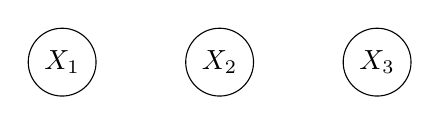
\begin{tikzpicture}
    \node[circle, draw] (X1) at (0,0) {$X_1$};
    \node[circle, draw] (X2) at (2,0) {$X_2$};
    \node[circle, draw] (X3) at (4,0) {$X_3$};
\end{tikzpicture}
\]

\newpage
\section{Variational Inference}
\subsection{Mean-Field Approximation for Multivariate Gaussians}
In this question, we’ll explore how accurate a Mean-Field approximation can be for an underlying multivariate Gaussian distribution. Assume we have observed data \( X \in \mathbb{R}^{2 \times n} \) where each column \( X_{\cdot,i} \triangleq x^{(i)} \in \mathbb{R}^2 \) is a sample that was drawn from a 2-dimensional Gaussian distribution \( x^{(i)} \sim p(\cdot; \mu, \Lambda^{-1}) \).

\[
p(x; \mu, \Lambda) = \mathcal{N} \left( 
\begin{bmatrix}
x_1 \\
x_2
\end{bmatrix}
;
\begin{bmatrix}
\mu_1 \\
\mu_2
\end{bmatrix}
,
\begin{bmatrix}
\Lambda_{11} & \Lambda_{12} \\
\Lambda_{21} & \Lambda_{22}
\end{bmatrix}^{-1}
\right)
\tag{1}
\]

Note here that we’re using the precision matrix \( \Lambda = \Sigma^{-1} \). An additional property of the precision matrix is that it is symmetric, so \( \Lambda_{12} = \Lambda_{21} \). (This is a convenient simplifying assumption.) We will approximate this 2-dimensional Gaussian with a mean field approximation, \( q(x) = q(x_1)q(x_2) \), the product of two 1-dimensional distributions \( q(x_1) \) and \( q(x_2) \). For now, we won’t assume any form for these distributions.

\begin{enumerate}
    \item \textbf{Short Answer:} Write down the equation for \( \log p(X) \). (For this question, you can leave all of the parameters in terms of vectors and matrices, not their subcomponents.)
    We approximate a 2D Gaussian distribution \(p(\mathbf{x}; \boldsymbol{\mu}, \boldsymbol{\Lambda})\) with a mean-field distribution \(q(\mathbf{x}) = q(x_1) q(x_2)\), where \(\mathbf{x} = [x_1, x_2]^T\), and answer questions about the log-probability, KL divergence, and numerical results.

\textbf{1. Log-Probability \(\log p(\mathbf{X})\)}:

For \(\mathbf{X} = [\mathbf{x}^{(1)}, \dots, \mathbf{x}^{(n)}]\), each \(\mathbf{x}^{(i)} \sim \mathcal{N}(\boldsymbol{\mu}, \boldsymbol{\Lambda}^{-1})\), the joint probability is:

\[
p(\mathbf{X}) = \prod_{i=1}^n \frac{|\boldsymbol{\Lambda}|^{1/2}}{(2\pi)} \exp\left( -\frac{1}{2} (\mathbf{x}^{(i)} - \boldsymbol{\mu})^T \boldsymbol{\Lambda} (\mathbf{x}^{(i)} - \boldsymbol{\mu}) \right)
\]

\[
\log p(\mathbf{X}) = \frac{n}{2} \log |\boldsymbol{\Lambda}| - n \log (2\pi) - \frac{1}{2} \sum_{i=1}^n (\mathbf{x}^{(i)} - \boldsymbol{\mu})^T \boldsymbol{\Lambda} (\mathbf{x}^{(i)} - \boldsymbol{\mu})
\]

\[
m_1 = \mu_1 - \Lambda_{11}^{-1} \Lambda_{12} (\mathbb{E}[x_2] - \mu_2) = 0 - 1 \cdot 0 \cdot (\mathbb{E}[x_2] - 0) = 0
\]
    \item \textbf{Short Answer:} Group together everything that involves \( X_1 \) and remove anything involving \( X_2 \). We claim that there exists some distribution \( q^*(X) = q^*(X_1)q^*(X_2) \) that minimizes the KL divergence \( q^* = \arg\min_q \text{KL}(q \| p) \). Furthermore, said distribution will have a component \( q^*(X_1) \) that will be proportional to the quantity you find below. Write that term that is proportional to \( q^*(X_1) \).
    \\\\ It can be shown that this implies that \( q(X_1) \) (and therefore \( q(X_2) \)) is a Gaussian distribution:
    \[
    q(x_1) = \mathcal{N} \left( x_1; m_1, \Lambda_{11}^{-1} \right)
    \]
    where 
    \[
    m_1 = \mu_1 - \Lambda_{11}^{-1} \Lambda_{12} \big(E[x_2] - \mu_2\big)
    \]
    Using these facts, we’d like to explore how well our approximation can model the underlying distribution.
    For a single sample, expand \(\log p(\mathbf{x})\):

\[
\log p(\mathbf{x}) = \frac{1}{2} \log |\boldsymbol{\Lambda}| - \log (2\pi) - \frac{1}{2} \begin{bmatrix} x_1 - \mu_1 \\ x_2 - \mu_2 \end{bmatrix}^T \begin{bmatrix} \Lambda_{11} & \Lambda_{12} \\ \Lambda_{12} & \Lambda_{22} \end{bmatrix} \begin{bmatrix} x_1 - \mu_1 \\ x_2 - \mu_2 \end{bmatrix}
\]

\[
= \frac{1}{2} \log |\boldsymbol{\Lambda}| - \log (2\pi) - \frac{1}{2} \left[ \Lambda_{11} (x_1 - \mu_1)^2 + 2 \Lambda_{12} (x_1 - \mu_1)(x_2 - \mu_2) + \Lambda_{22} (x_2 - \mu_2)^2 \right]
\]

Terms involving \(x_1\):

\[
-\frac{1}{2} \left[ \Lambda_{11} (x_1 - \mu_1)^2 + 2 \Lambda_{12} (x_1 - \mu_1)(x_2 - \mu_2) \right]
\]

The term proportional to \(q^*(x_1)\) is:

\[
\exp\left( -\frac{1}{2} \left[ \Lambda_{11} (x_1 - \mu_1)^2 + 2 \Lambda_{12} (x_1 - \mu_1)(x_2 - \mu_2) \right] \right)
\]

    \item Suppose the parameters of the true distribution are 
    \[
    \mu = 
    \begin{bmatrix}
    0 \\
    0
    \end{bmatrix}
    \quad \text{and} \quad
    \Lambda = 
    \begin{bmatrix}
    1 & 0 \\
    0 & \frac{1}{4}
    \end{bmatrix}.
    \]
        \begin{enumerate}
            \item[(a)] \textbf{Numerical Answer:} What is the value of the mean of the Gaussian for \( q^*(X_1) \)?
\[
m_1 = \mu_1 - \Lambda_{11}^{-1} \Lambda_{12} (\mathbb{E}[x_2] - \mu_2) = 0 - 1 \cdot 0 \cdot (\mathbb{E}[x_2] - 0) = 0
\]
            \item[(b)] (2 points) \textbf{Numerical Answer:} What is the value of the variance of the Gaussian for \( q^*(X_1) \)?
\[
\Lambda_{11}^{-1} = 1^{-1} = 1
\]
            \item[(c)] (2 points) \textbf{Numerical Answer:} What is the value of the mean of the Gaussian for \( q^*(X_2) \)?
            \[
m_2 = \mu_2 - \Lambda_{22}^{-1} \Lambda_{12} (\mathbb{E}[x_1] - \mu_1) = 0 - 4 \cdot 0 \cdot (\mathbb{E}[x_1] - 0) = 0
\]
            \item[(d)] (2 points) \textbf{Numerical Answer:} What is the value of the variance of the Gaussian for \( q^*(X_2) \)?
\[
\Lambda_{22}^{-1} = (1/4)^{-1} = 4
\]
            \item[(e)] (5 points) \textbf{Plot:} Provide a computer-generated contour plot to show the result of our approximation \( q^*(X) \) and the true underlying Gaussian \( p(X; \mu, \Lambda) \) for the parameters given above.
            Since \(\Lambda_{12} = 0\), \(p(\mathbf{x}) = \mathcal{N}(\mathbf{x}; [0,0]^T, \begin{bmatrix} 1 & 0 \\ 0 & 4 \end{bmatrix})\) has no correlation, and \(q^*(\mathbf{x}) = \mathcal{N}(x_1; 0, 1) \mathcal{N}(x_2; 0, 4) = p(\mathbf{x})\). The contours are identical, showing axis-aligned ellipses (variance 1 in \(x_1\), 4 in \(x_2\)).

            \[
            \begin{tikzpicture}
                \draw[->] (-3,0) -- (3,0) node[right] {$x_1$};
                \draw[->] (0,-5) -- (0,5) node[above] {$x_2$};
                \draw[blue, thick] (0,0) ellipse (1 and 4) node[above right, blue] {$p(\mathbf{x}), q^*(\mathbf{x})$};
            \end{tikzpicture}
            \]
        \end{enumerate}
    \item  Suppose the parameters of the true distribution are 
    \[
    \mu = 
    \begin{bmatrix}
    1 \\
    2
    \end{bmatrix}
    \quad \text{and} \quad
    \Lambda = 
    \begin{bmatrix}
    \frac{2}{3} & -\frac{1}{3} \\
    -\frac{1}{3} & \frac{2}{3}
    \end{bmatrix}.
    \]
    
        \begin{enumerate}
            \item[(a)] (2 points) \textbf{Numerical Answer:} What is the value of the mean of the Gaussian for \( q^*(X_1) \)?
  \[
m_1 = \mu_1 - \Lambda_{11}^{-1} \Lambda_{12} (\mathbb{E}[x_2] - \mu_2), \quad \Lambda_{11}^{-1} = \frac{3}{2}
\]
Assume \(\mathbb{E}[x_2] = m_2\). Iteratively:

\[
m_1 = 1 - \frac{3}{2} \cdot \left(-\frac{1}{3}\right) (m_2 - 2) = 1 + \frac{1}{2} (m_2 - 2)
\]
            \item[(b)] (2 points) \textbf{Numerical Answer:} What is the value of the variance of the Gaussian for \( q^*(X_1) \)?
            \[
\Lambda_{11}^{-1} = \frac{3}{2}
\]
            \item[(c)] (2 points) \textbf{Numerical Answer:} What is the value of the mean of the Gaussian for \( q^*(X_2) \)?
           \[
m_2 = \mu_2 - \Lambda_{22}^{-1} \Lambda_{12} (\mathbb{E}[x_1] - \mu_1), \quad \Lambda_{22}^{-1} = \frac{3}{2}
\]

\[
m_2 = 2 - \frac{3}{2} \cdot \left(-\frac{1}{3}\right) (m_1 - 1) = 2 + \frac{1}{2} (m_1 - 1)
\]

Solve: \(m_1 = 1 + \frac{1}{2} (m_2 - 2)\), \(m_2 = 2 + \frac{1}{2} (m_1 - 1)\).

\[
m_2 = 2 + \frac{1}{2} \left( 1 + \frac{1}{2} (m_2 - 2) - 1 \right) = 2 + \frac{1}{4} (m_2 - 2)
\]

\[
m_2 = 2 + \frac{1}{4} m_2 - \frac{1}{2}, \quad \frac{3}{4} m_2 = \frac{3}{2}, \quad m_2 = 2
\]

\[
m_1 = 1 + \frac{1}{2} (2 - 2) = 1
\]
            \item[(d)] (2 points) \textbf{Numerical Answer:} What is the value of the variance of the Gaussian for \( q^*(X_2) \)?
\[
\Lambda_{22}^{-1} = \frac{3}{2}
\]
            \item[(e)] (5 points) \textbf{Plot:} Provide a computer-generated contour plot to show the result of our approximation \( q^*(X) \) and the true underlying Gaussian \( p(X; \mu, \Lambda) \) for the parameters given above.
            \(p(\mathbf{x})\): \(\mathcal{N}(\mathbf{x}; [1,2]^T, \begin{bmatrix} 2 & 1 \\ 1 & 2 \end{bmatrix})\), with correlation.

\(q^*(\mathbf{x})\): \(\mathcal{N}(x_1; 1, \frac{3}{2}) \mathcal{N}(x_2; 2, \frac{3}{2})\), axis-aligned.

\[
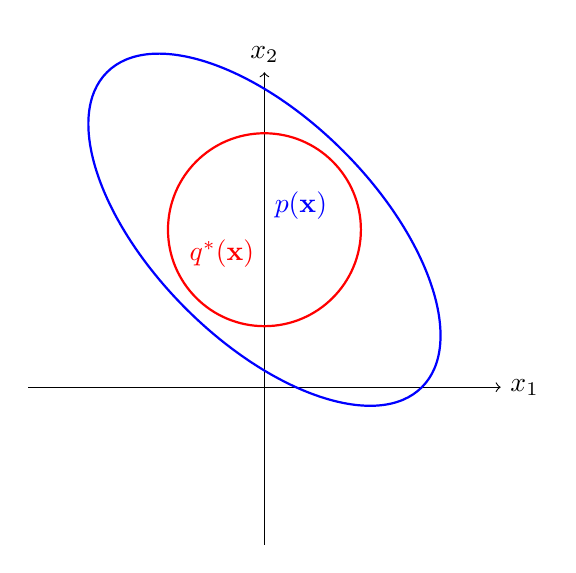
\begin{tikzpicture}
    \draw[->] (-2,0) -- (4,0) node[right] {$x_1$};
    \draw[->] (1,-2) -- (1,4) node[above] {$x_2$};
    \draw[blue, thick, rotate around={45:(1,2)}] (1,2) ellipse (1.414 and 2.828) node[above right, blue] {$p(\mathbf{x})$};
    \draw[red, thick] (1,2) ellipse (1.225 and 1.225) node[below left, red] {$q^*(\mathbf{x})$};
\end{tikzpicture}
\]
        \end{enumerate}
    \item (2 points) Describe in words how the plots you generated provide insight into the behavior of minimization of
    KL(q||p) with regards to the low probability and high probability regions of the true vs. approximate distributions.

    In Case 1 (\(\Lambda_{12} = 0\)), \(p(\mathbf{x})\) has no correlation, so \(q^*(\mathbf{x}) = p(\mathbf{x})\), and contours match perfectly (\(\text{KL}(q \| p) = 0\)). High- and low-probability regions align.

In Case 2 (\(\Lambda_{12} \neq 0\)), \(p(\mathbf{x})\) has correlation (tilted ellipses), but \(q^*(\mathbf{x})\) assumes independence (axis-aligned). Minimizing \(\text{KL}(q \| p)\) matches high-probability regions well, but \(q^*\) overestimates low-probability tails, as seen in the broader, misaligned contours of \(q^*\).
\end{enumerate}

\subsection{Variational Inference vs. Monte Carlo Methods}

Let’s end with a brief comparison between variational methods and MCMC methods. We have seen that both
classes of methods can be used for learning in scenarios involving latent variables, but both have their own sets of
advantages and disadvantages. For each of the following statements, specify whether they apply more suitably to
VI or MCMC methods:

\begin{enumerate}
    \item (2 points) Transforms inference into optimization problems.\\
    \(\bigcirc\) Variational Inference \(\checkmark\) \\
    \(\bigcirc\) MCMC
    \item (2 points) Is easier to integrate with back-propagation.\\
    \(\bigcirc\) Variational Inference \(\checkmark\) \\
    \(\bigcirc\) MCMC
    \item (2 points) Involves more stochasticity.\\
    \(\bigcirc\) Variational Inference \\
    \(\bigcirc\) MCMC \(\checkmark\)
    \item (2 points) Converges to the true distribution.\\
    \(\bigcirc\) Variational Inference \\
    \(\bigcirc\) MCMC \(\checkmark\)
    \item (2 points) Is higher variance under limited computational resources.\\
    \(\bigcirc\) Variational Inference  \\
    \(\bigcirc\) MCMC \(\checkmark\)
\end{enumerate}

\end{document}
